\documentclass[10pt,a4paper]{article}
\usepackage[margin=2.2cm]{geometry}
\usepackage[T1]{fontenc}
\usepackage{mathpazo}
\usepackage{microtype}
\usepackage{amsmath}
\usepackage{graphicx}
\usepackage{booktabs}
\usepackage{caption}
\usepackage[hidelinks]{hyperref}
\usepackage{cleveref}
\graphicspath{{../figures/}}
\captionsetup{font=small,labelfont=bf}
\setlength{\parskip}{3pt}

\title{\vspace{-1.5em}\Large\bfseries When Is a PINN Worth It?\\[2pt]
\large Boundary Enforcement and Classical Baselines for the 1D Heat Equation}
\author{Sattwik Singh\\
\small Department of Electrical Engineering, Indian Institute of Technology Delhi}
\date{\small November 2026}

\begin{document}
\maketitle

\begin{abstract}
\noindent Physics-informed neural networks (PINNs) can solve differential equations without a mesh, but their accuracy depends on training choices that classical solvers do not have. We study one such choice, how boundary and initial conditions are imposed, on the 1D heat equation with Dirichlet, Neumann and mixed boundaries, where exact solutions are available. Over five seeds, building the conditions into the network reduced median relative $L^2$ error by a factor of 2.2 to 4.4 compared with the best penalty weight, reaching 0.003--0.005\%. Larger penalty weights lowered the boundary violation but raised the overall error. The advantage did not hold everywhere: on a rapidly decaying eighth eigenmode, hard enforcement failed and the soft PINN was also unreliable. Crank--Nicolson matched the best PINN accuracy in about 2\,ms, against about 100\,s of training, and also recovered the diffusivity from noisy sensors more accurately. On this problem, the PINN offers no practical advantage over a classical solver.
\end{abstract}

\section{Introduction}
PINNs train a network to satisfy a differential equation by penalising its residual at sampled points~\cite{raissi2019}. The usual loss adds penalty terms for the boundary and initial conditions, and the balance between these terms can make training difficult~\cite{wang2021,krishnapriyan2021}. An alternative is to transform the network output so that the conditions hold exactly~\cite{lagaris1998,sukumar2022}.

The heat equation is a useful test case because it is simple enough to remove most sources of doubt: exact solutions exist and classical solvers are excellent. Any weakness that appears here cannot be blamed on the problem being hard. We ask three questions. How much does enforcement strategy matter? How does the best PINN compare with finite differences on accuracy and cost? Where does the method fail?

This work extends an earlier supervised project, in which a soft-constrained PINN reached about 5\% relative $L^2$ error and boundary treatment appeared to be the most important factor. Here that observation is tested in a controlled, multi-seed study.

\section{Problem and methods}
\paragraph{Problem.} We solve $u_t=\alpha u_{xx}$ on $x\in[0,1]$, $t\in[0,1]$, with $\alpha=0.1$ and homogeneous Dirichlet, Neumann or mixed ($u(0,t)=0$, $u_x(1,t)=0$) boundaries. The initial condition combines the first two eigenmodes with amplitudes 1 and 0.5, for example $u(x,t)=e^{-\alpha\pi^2 t}\sin\pi x+0.5\,e^{-4\alpha\pi^2 t}\sin 2\pi x$ in the Dirichlet case.

\paragraph{Soft and hard enforcement.} The soft PINN minimises $\mathcal{L}=\mathcal{L}_{\mathrm{pde}}+w(\mathcal{L}_{\mathrm{bc}}+\mathcal{L}_{\mathrm{ic}})$ for $w\in\{1,10,100\}$. The hard PINN minimises $\mathcal{L}_{\mathrm{pde}}$ alone, using
\begin{equation}
\hat{u}(x,t)=u_0(x)+t\,g(x)\,N_\theta(\phi(x),t),
\end{equation}
which matches the initial condition for all network parameters $\theta$. For Dirichlet boundaries $g=4x(1-x)$. For Neumann boundaries $g=1$ and $\phi=\cos\pi x$, so that $\hat{u}_x$ vanishes at both ends. For mixed boundaries $g=\phi=\sin(\pi x/2)$, up to a rescaling of the network input.

\paragraph{Training.} The network is a tanh MLP with four hidden layers of 50 units in double precision. Training uses 3000 Adam steps with cosine decay from $10^{-3}$, then up to 1000 L-BFGS iterations on 2000 fixed Sobol collocation points, with 200 boundary and 200 initial points for the soft loss. No hyperparameter search was performed.

\paragraph{Baselines and metrics.} FTCS and Crank--Nicolson use second-order central differences, with mirrored ghost nodes at Neumann boundaries. FTCS runs at a stability number of about 0.4, and Crank--Nicolson uses $\Delta t=\Delta x$. Error is the relative $L^2$ norm over space and time against the exact solution, computed on a $201\times101$ grid for PINNs and on each solver's own grid for finite differences. Runtimes use one CPU thread. All 105 training runs and the code are available in the project repository, and unit tests confirm the exact solutions, the hard constraints, and the expected second-order convergence of Crank--Nicolson.

\section{Results}
\paragraph{Boundary enforcement.} Hard enforcement gave the lowest median error for every boundary type (\cref{tab:boundary,fig:boundary}), with no overlap between its five seeds and those of any soft configuration. The gain was largest for Dirichlet boundaries (4.4 times) and smallest for Neumann (2.2 times). The error fields in \cref{fig:fields} show soft errors spread across the domain, not concentrated at the boundary. Raising $w$ to 100 reduced the boundary violation but gave the worst overall error in all three cases, so a smaller boundary residual did not mean a better solution. L-BFGS mattered greatly: it lowered the hard PINN's median error by a factor of 11 to 18 after Adam.

\begin{table}[!htbp]
\centering\small
\caption{Median relative $L^2$ error (\%) over five seeds. The last column is the improvement of hard enforcement over the best soft weight.}
\label{tab:boundary}
\begin{tabular}{lccccc}
\toprule
Boundary & $w=1$ & $w=10$ & $w=100$ & Hard & Improvement\\
\midrule
Dirichlet & 0.0232 & 0.0200 & 0.0565 & \textbf{0.0046} & 4.4$\times$\\
Neumann & 0.0111 & 0.0292 & 0.0964 & \textbf{0.0051} & 2.2$\times$\\
Mixed & 0.0084 & 0.0104 & 0.0269 & \textbf{0.0027} & 3.1$\times$\\
\bottomrule
\end{tabular}
\end{table}

\begin{figure}[!htbp]
\centering
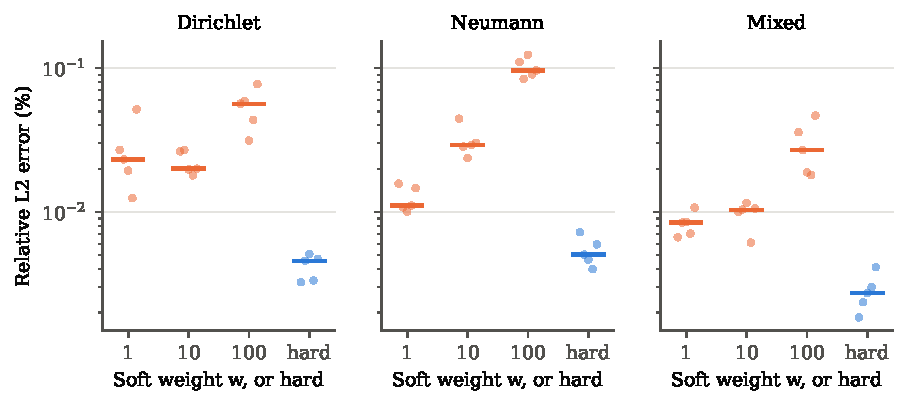
\includegraphics[width=0.76\linewidth]{boundary_enforcement.pdf}
\caption{Error for each seed (dots) and the median (bar). Note the logarithmic scale.}
\label{fig:boundary}
\end{figure}

\begin{figure}[!htbp]
\centering
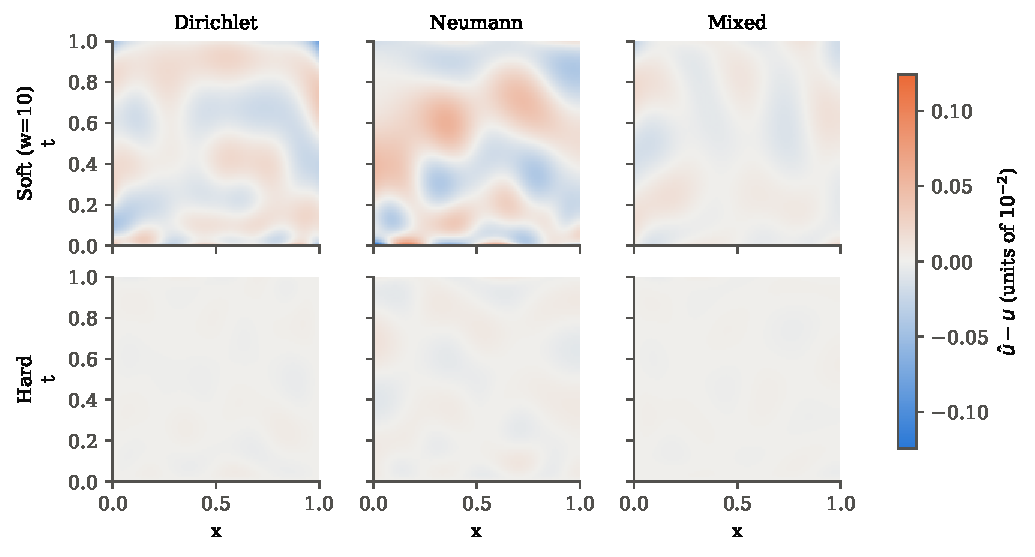
\includegraphics[width=0.72\linewidth]{error_fields.pdf}
\caption{Signed error for seed 0, on a shared colour scale. Axes show position $x$ and time $t$.}
\label{fig:fields}
\end{figure}

\paragraph{Cost against finite differences.} \Cref{fig:cost} shows the Dirichlet case. Crank--Nicolson reached 0.0018\% with 160 cells in 1.9\,ms, better than the hard PINN's 0.0046\% after 108\,s, or about 57{,}000 times faster. With 640 cells it reached 0.00012\% in 11\,ms. FTCS was also ahead of the PINN once refined, though its stability limit makes it slower than Crank--Nicolson at high resolution.

\begin{figure}[!htbp]
\centering
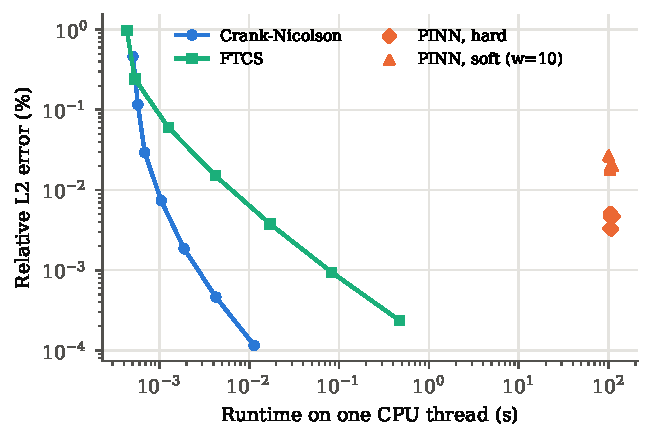
\includegraphics[width=0.47\linewidth]{accuracy_vs_runtime.pdf}
\caption{Error against runtime for the Dirichlet problem. Lines show grid refinement from 10 to 640 cells.}
\label{fig:cost}
\end{figure}

\paragraph{Limits of the PINN.} We then trained on single eigenmodes (\cref{fig:frequency}, left). Hard-PINN error stayed at or below about 0.01\% for modes 1 and 2, rose to 0.24--0.42\% for mode 4, and failed for mode 8 at 19--1154\%. Soft enforcement ($w=10$) was similar at mode 4 (0.41--0.61\%) and better at mode 8 (5.7--60\%), so the advantage of hard enforcement is conditional, and neither version was reliable there. Mode 8 decays at rate $\alpha(8\pi)^2\approx63$, so the solution vanishes within the first few percent of the time window. We suspect the factor of $t$ in Eq.~(1) contributes, because the network must output large values at early times to cancel $u_0$, but we have not tested this. Spectral bias~\cite{rahaman2019} and the failure modes of~\cite{krishnapriyan2021} are other possible causes.

Accuracy also depended on collocation count (\cref{fig:frequency}, right). Median error fell from 0.16\% with 50 points to 0.0076\% with 200 and 0.0036\% with 1000, then showed no further gain at 4000 (0.0045\%) despite about four times the runtime.

\begin{figure}[!htbp]
\centering
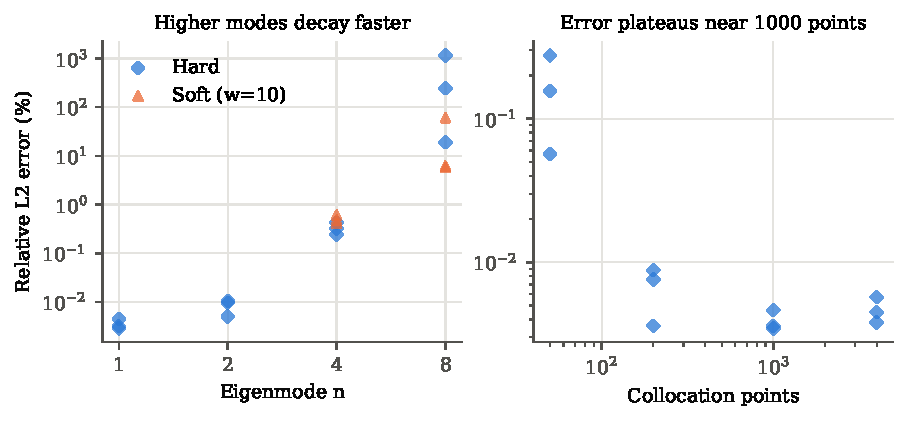
\includegraphics[width=0.76\linewidth]{frequency_collocation.pdf}
\caption{Left: single-eigenmode problems. Right: hard PINN against collocation count on the Dirichlet problem. Each marker is one seed.}
\label{fig:frequency}
\end{figure}

\paragraph{Estimating the diffusivity.} Inverse problems are often proposed as a natural use of PINNs. We estimated $\alpha$ from 50 readings at five sensor positions and ten times, with Gaussian noise relative to the signal's RMS, starting the PINN from $\alpha=0.3$. As a baseline, we minimised the data misfit over $\alpha$ with a one-dimensional bounded search around a Crank--Nicolson solve (\cref{tab:inverse,fig:inverse}). The PINN was slightly better on clean data, likely because the baseline carries discretisation error. With noise, the classical fit was about twice as accurate, the PINN's estimates were consistently low at 5\% noise, and the classical fit took 23\,ms against about 107\,s.

\begin{table}[!htbp]
\centering\small
\caption{Recovery of $\alpha=0.1$ over five noise seeds, as mean absolute error (\%).}
\label{tab:inverse}
\begin{tabular}{lccc}
\toprule
Noise & PINN & Crank--Nicolson fit & Median runtime (PINN / fit)\\
\midrule
0\% & \textbf{0.004} & 0.011 & 105\,s / 23\,ms\\
1\% & 0.35 & \textbf{0.18} & 107\,s / 23\,ms\\
5\% & 2.14 & \textbf{0.91} & 109\,s / 22\,ms\\
\bottomrule
\end{tabular}
\end{table}

\begin{figure}[!htbp]
\centering
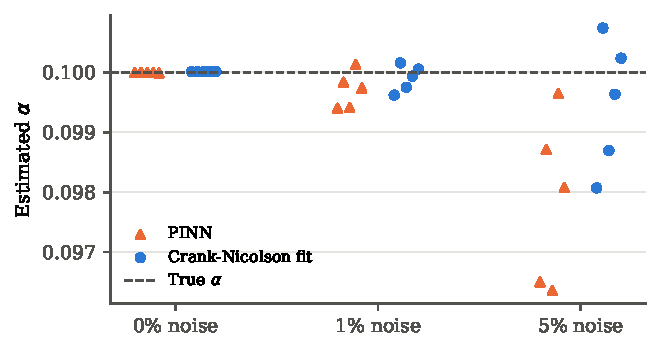
\includegraphics[width=0.47\linewidth]{inverse_alpha.pdf}
\caption{Estimated diffusivity for each noise seed.}
\label{fig:inverse}
\end{figure}

\section{Discussion}
The earlier observation holds up: enforcement strategy strongly affects accuracy, and the simplest remedy is to remove the penalty rather than tune it. Two qualifications matter. Hard enforcement helped on smooth problems but was not robust for fast decay. And a penalty that lowers boundary error does not necessarily lower total error.

The comparison with finite differences should be read within its scope. This is a low-dimensional, linear problem on a simple domain, which is where classical solvers are strongest. It says nothing about high-dimensional or irregular problems, where the balance may differ. Other limits are the small number of seeds, the single untuned network, the single fixed data weight in the inverse problem, and the use of a one-parameter classical fit, which would be harder to apply if the unknown were a whole function. These last cases are where PINNs might still earn their cost, and they are the natural next step, along with testing a time factor suited to fast decay.

\section{Conclusion}
For the 1D heat equation, exact enforcement of boundary conditions made PINNs two to four times more accurate on smooth solutions, but not on a fast-decaying mode. Crank--Nicolson was still orders of magnitude faster at equal accuracy and was more reliable on the noisy inverse problem. The main lesson is that a PINN result needs a classical baseline and an explicit test of where it breaks.

\paragraph{Acknowledgements and AI use.} The original project was carried out under Prof.\ Abhishek M.\ Iyer at IIT Delhi. The code and this report for the present study were developed with AI assistance (Claude). The author directed the work and takes responsibility for the results.

\begin{thebibliography}{9}\small\setlength{\itemsep}{0pt}
\bibitem{raissi2019} M.~Raissi, P.~Perdikaris, G.~E.~Karniadakis. Physics-informed neural networks. \emph{J.\ Comput.\ Phys.} 378:686--707, 2019.
\bibitem{lagaris1998} I.~E.~Lagaris, A.~Likas, D.~I.~Fotiadis. Artificial neural networks for solving ordinary and partial differential equations. \emph{IEEE Trans.\ Neural Netw.} 9(5):987--1000, 1998.
\bibitem{wang2021} S.~Wang, Y.~Teng, P.~Perdikaris. Understanding and mitigating gradient flow pathologies in physics-informed neural networks. \emph{SIAM J.\ Sci.\ Comput.} 43(5):A3055--A3081, 2021.
\bibitem{krishnapriyan2021} A.~S.~Krishnapriyan, A.~Gupta, S.~Zhu, R.~M.~Kirby, M.~W.~Mahoney. Characterizing possible failure modes in physics-informed neural networks. \emph{NeurIPS} 34, 2021.
\bibitem{sukumar2022} N.~Sukumar, A.~Srivastava. Exact imposition of boundary conditions with distance functions in physics-informed deep neural networks. \emph{Comput.\ Methods Appl.\ Mech.\ Eng.} 389:114333, 2022.
\bibitem{rahaman2019} N.~Rahaman et al. On the spectral bias of neural networks. \emph{ICML}, PMLR 97:5301--5310, 2019.
\end{thebibliography}
\end{document}
